\section{Methods}


\subsection{Experimental}

\begin{figure}[h]
    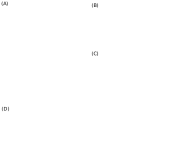
\includegraphics[width=\linewidth]{\repodir/figures/output/Fig_expt_setup.png} 
    \caption{Process flow diagram of the system.}
\end{figure}

\begin{itemize}
\item Determine kr vs nK, position, laser power
\item Absorption spectroscopy for nK
\item Microwave scattering (MWS) for kr 
\end{itemize}

\subsubsection{Microwave scattering modeling}

 

\begin{figure}[h]
    \includegraphics[width=\linewidth]{\repodir/experiment/analysis/mws/output/figures/fit_mws_dnent.png} 
    \includegraphics[width=\linewidth]{\repodir/experiment/analysis/mws/output/figures/fit_mws_exp.png} 
    \caption{Process flow diagram of the system.}
\end{figure}


We determine the state of charge with a kinetic model.

\begin{equation}
    \frac{d\Delta n_e}{dt} = - k_r [2 n_{K+,0}\Delta n_e + \Delta{n_e}^2]
\end{equation}

\section{Cantera}

Assessing viability in hypothetical conditions using kr value

\begin{figure}[h]
    \includegraphics[width=\linewidth]{\repodir/modeling/analysis/output/alpha_curve_demo.png} 
    \includegraphics[width=\linewidth]{\repodir/modeling/analysis/output/alpha_curve_analysis_lbk.png} 
    \caption{Process flow diagram of the system.}
\end{figure}

\section{CFD}

CFD modeling 

\begin{itemize}
\item nK+ for MWS kr determination
\item CFD results at goldilocks need examination
\item nK vs position profile, for line integral determination of nK
\item Methodology is not developed yet. 
\end{itemize}
